\problemname{Dreamcatcher}

\illustration{0.28}{illustration.jpg}{
	Pixabay Content Licence by wal\_172619 on \href{https://pixabay.com/photos/dream-catcher-decoration-5731922/}{Pixabay}
}

Lately, you are plagued by horrifying nightmares.
In those dreams, a swarm of angry Fenwick bees chases you around a tree with heavy and light branches.
You hate getting stung by their fiddling bits.
Therefore, you decided to build a dreamcatcher three days ago,
but the process is tricky, and you cannot figure out the details.

Planning your dreamcatcher became so stressful that you spent the last three nights awake,
thinking about long strings of yarn, Carmichael numbers, and geometry.
The only progress so far is some incomprehensible drawings (see Figure~\ref{fig:dreamcatcher}) and the observation
that the length of a chord that spans $\theta$ degrees of a circle with radius $r$ is $2r\cdot\sin(\theta/2)$.
But how is this going to help?
You would rather have the dreams about Fenwick bees again than being tormented by this dreadful project for one more day.
You need to solve this \emph{now}!

\begin{figure}[h]
	\centering
	\hfill
	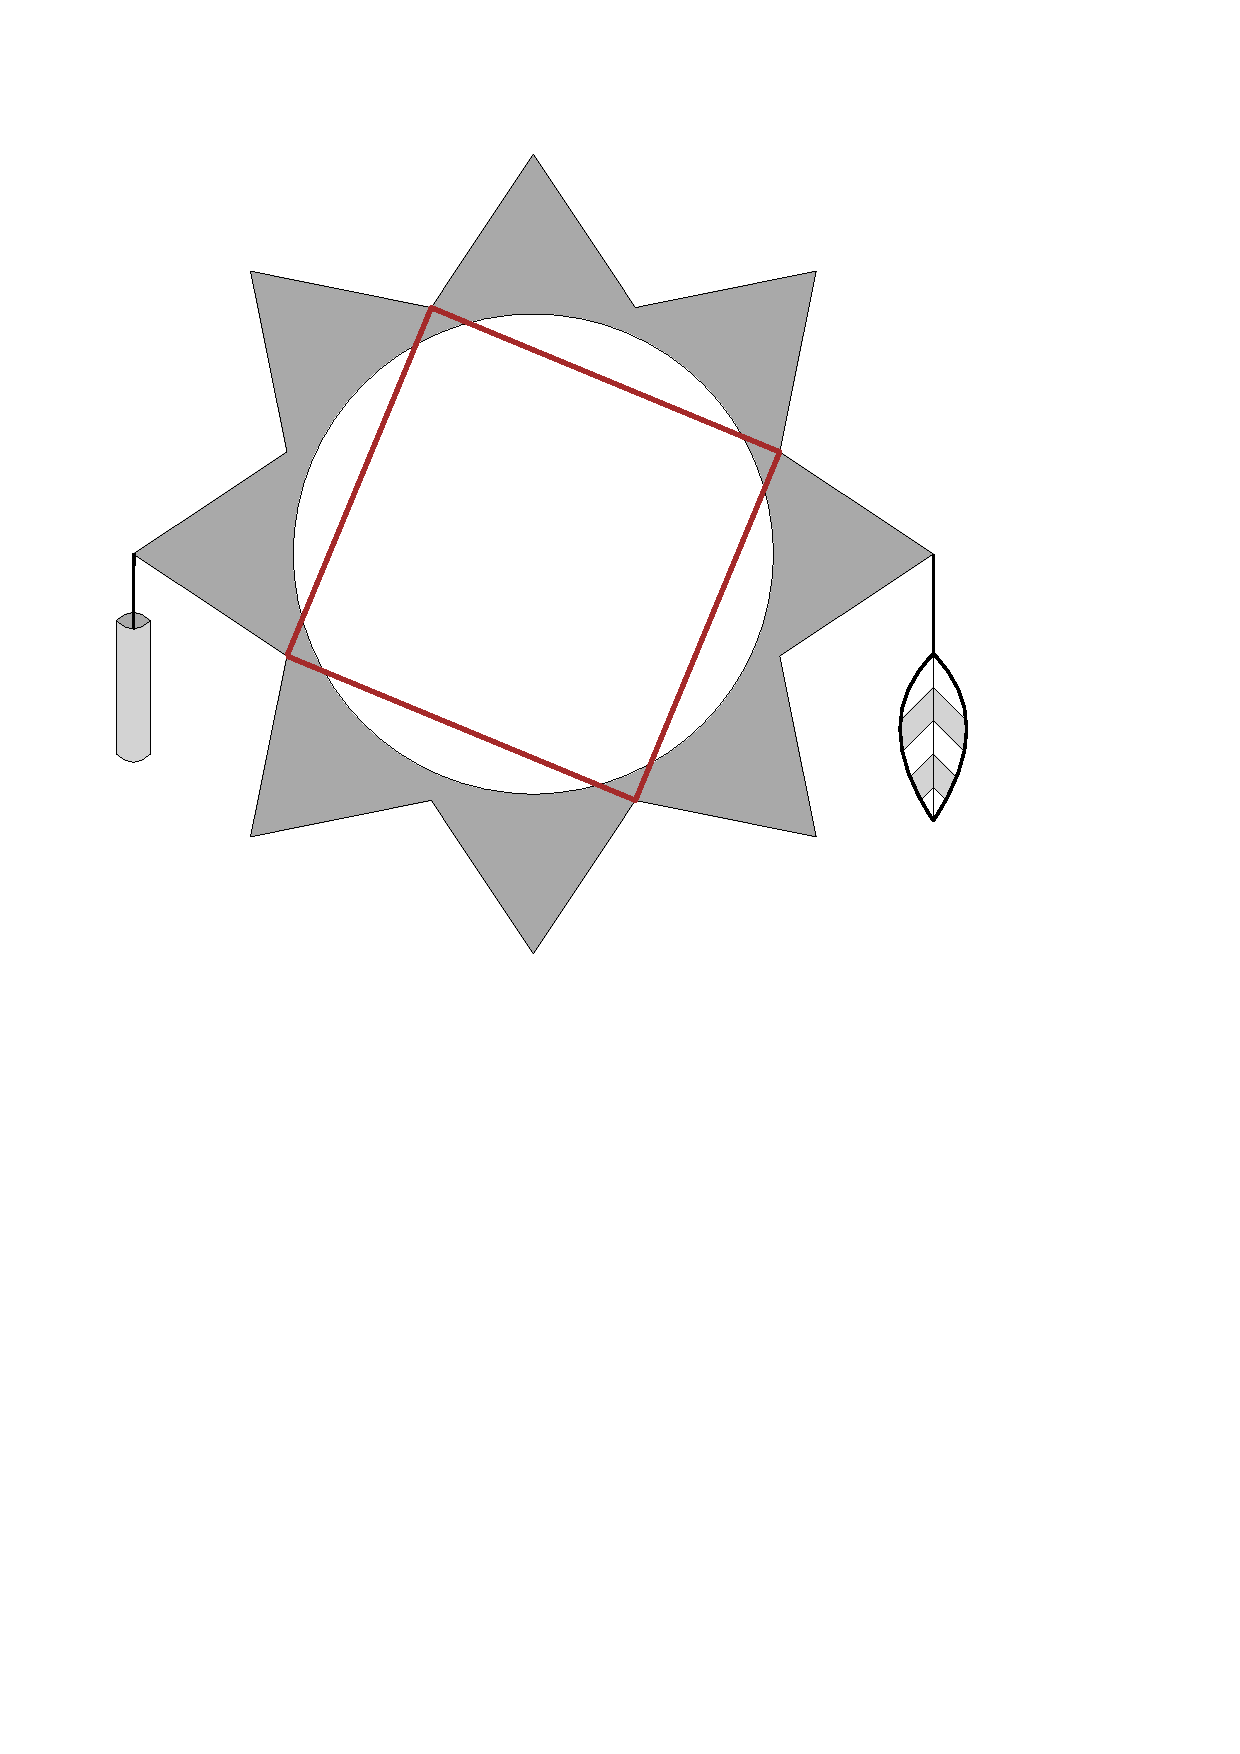
\includegraphics[width=3.5cm]{figure-n8-k2.pdf}
	\hfill
	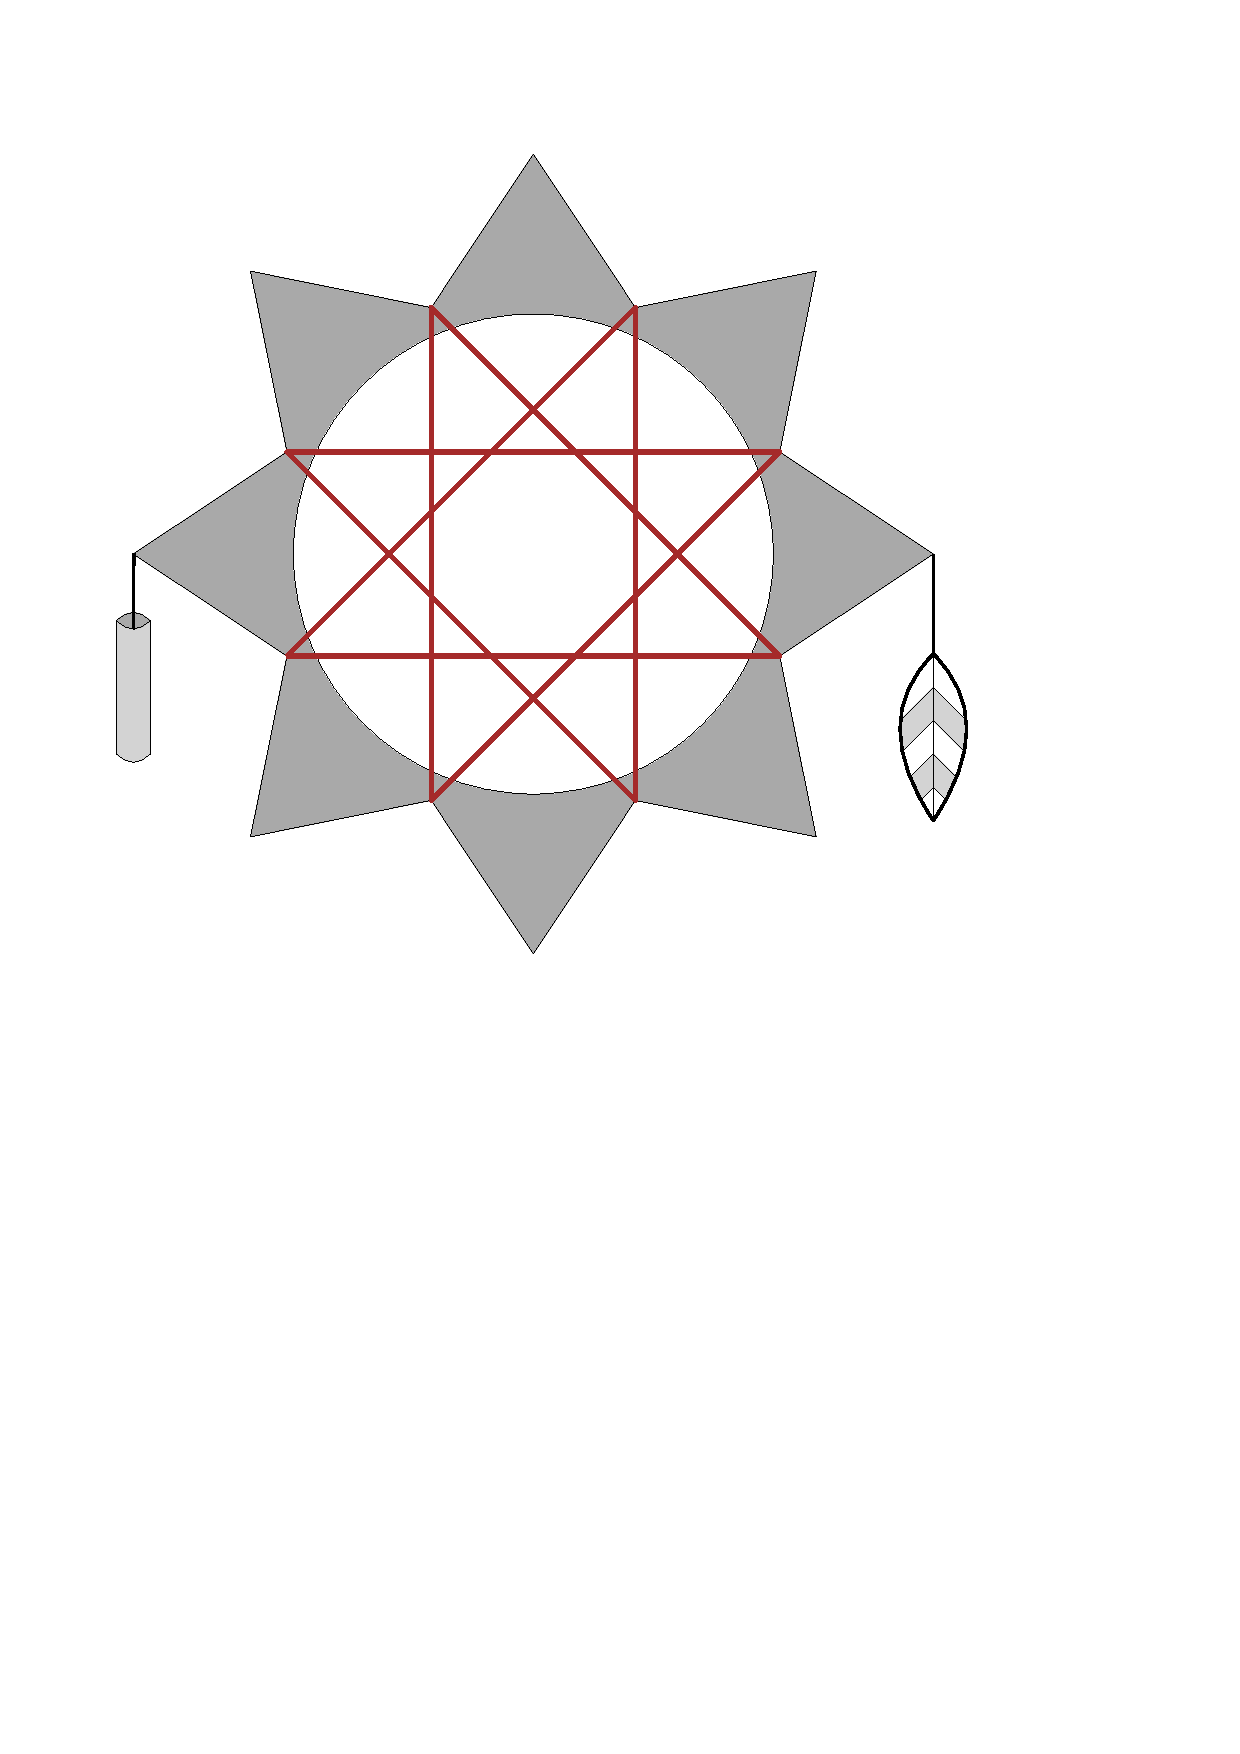
\includegraphics[width=3.5cm]{figure-n8-k3.pdf}
	\hfill
	\hfill% Silly LaTeX, requiring \hfill twice at the end of a line

	\caption{
        A dreamcatcher with $8$ notches, showing two ways of wrapping it in a string of yarn.
        The dreamcatcher on the left spans $2$ notches per chord, while the
        dreamcatcher on the right spans $3$ notches per chord.
		%Assuming a radius of $1$, each chord has a length of $2\sin(\pi \cdot \frac{3}{8})\approx 1.85$.
    }
	\label{fig:dreamcatcher}
\end{figure}


To build a dreamcatcher, you take a wheel with $n$ evenly spaced notches, numbered from $1$ to $n$.
You wrap a string of yarn around this wheel, spanning $k$ notches per chord:
starting at notch $1$, you repeatedly connect the yarn $k$ notches ahead until you reach notch $1$ again.
For example, with $n=8$ and $k=3$, you would go from notch $1$ to $4$, then $7$, $2$, $5$, $8$, $3$, $6$, $1$.

A dreamcatcher's effectiveness depends on the amount of used yarn.
You need to choose $k$, the number of notches to span per chord, such that the total length of yarn is maximized.
The answer does not depend on the radius of the dreamcatcher.

% E.g.
% For n=12 and k=8 the yarn connects 1,9,5,1 for a total of 12 yarn-units used.
% For n=3 and k=2 the yarn connects 1,3,2,1 for a total of 4 yarn-units used.

\begin{Input}
The input consists of:
\begin{itemize}
    \item One line with an integer $n$ ($3\leq n\leq 10^9$), the number of notches on the wheel.
\end{itemize}
\end{Input}

\begin{Output}
    Output an integer $k$ ($1\leq k < n$) that maximizes the length of used yarn when spanning $k$~notches per chord.

    If there are multiple valid solutions, you may output any one of them.
\end{Output}
